\section{模型检验与评价}

\subsection{模型检验}

\subsubsection*{鲁棒性分析}

为检验模型对判别阈值选取的敏感程度，本文将预测概率阈值从 0.1
逐步调整至 0.8，观察召回率与精确率的变化轨迹，如图
\ref{fig:threshold} 所示。

\begin{figure}[H]
    \centering
    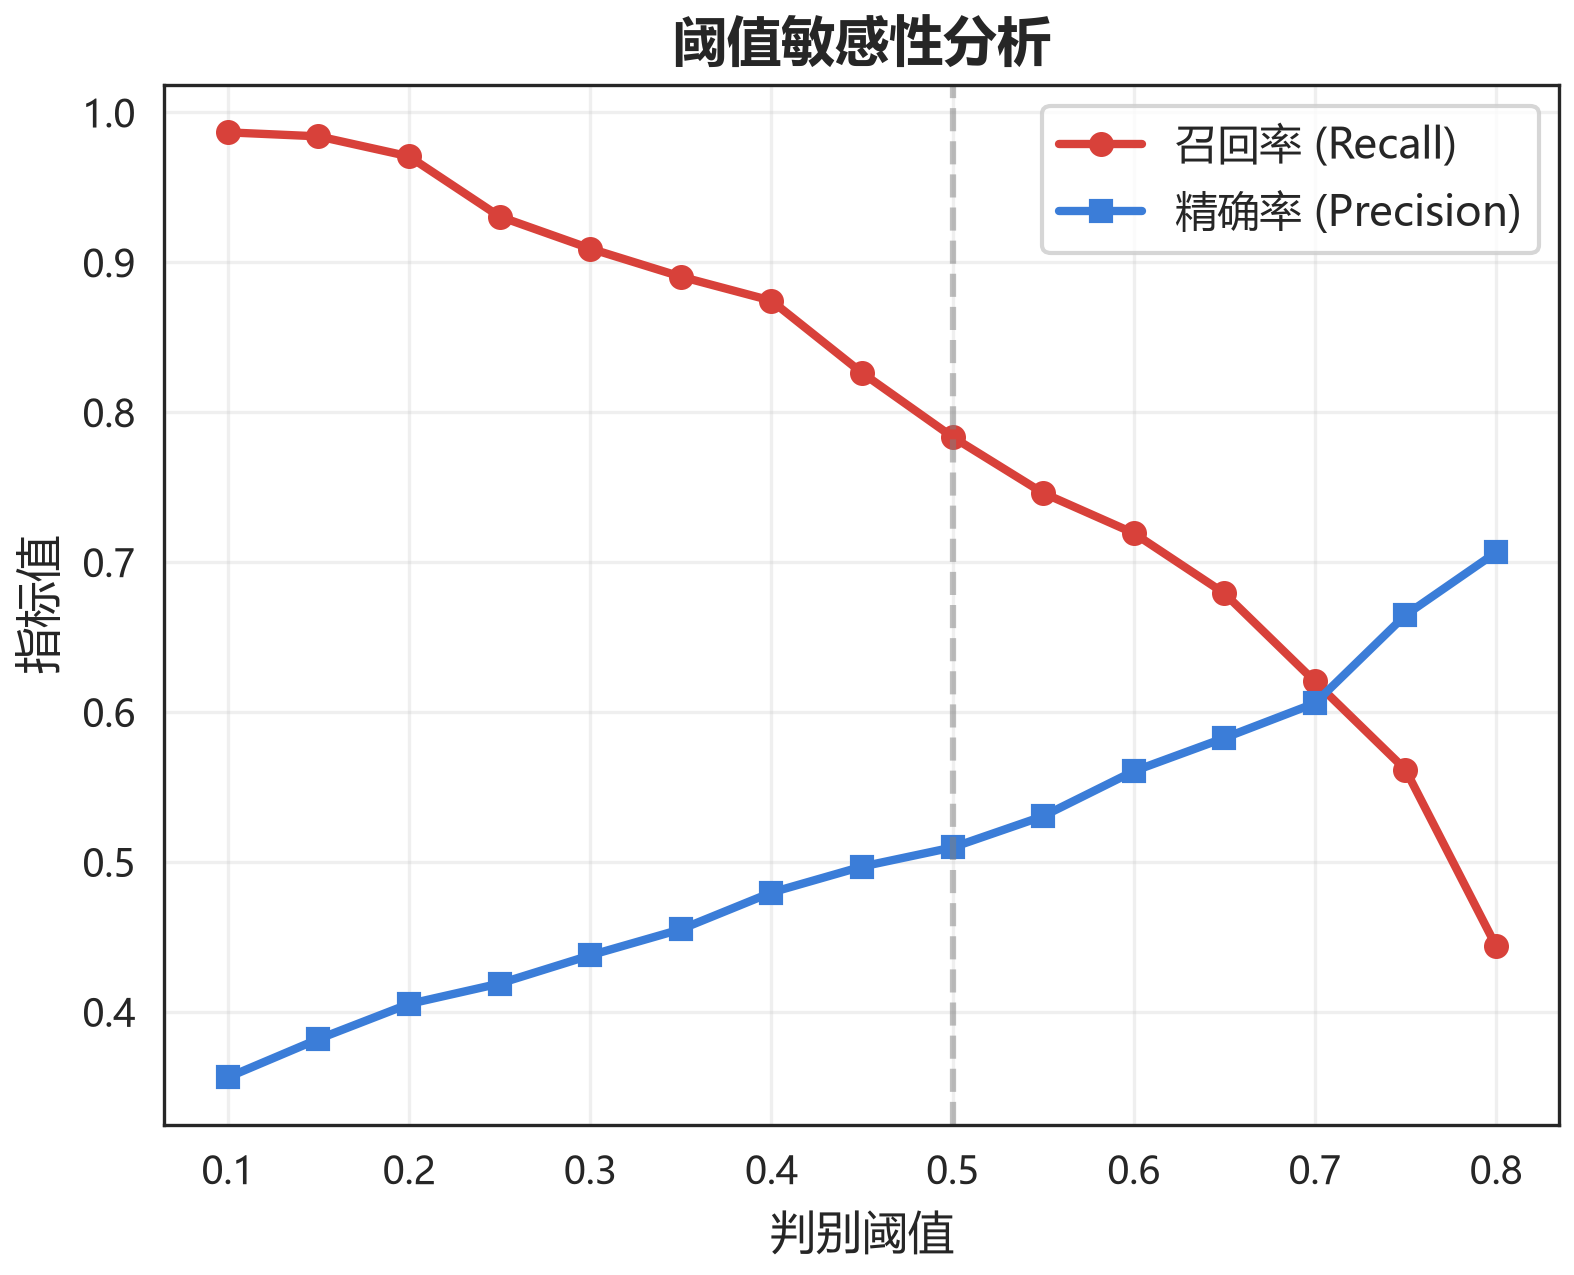
\includegraphics[width=0.7\textwidth]{figures/threshold_analysis.png}
    \caption{阈值敏感性分析}
    \label{fig:threshold}
\end{figure}

从图 \ref{fig:threshold} 可以看出，随着阈值从 0.1 升高到 0.8，
召回率单调下降（从 0.99 降至 0.44），精确率则单调上升
（从 0.36 升至 0.71），两者在阈值 0.5 附近形成交叉。
在 0.4-0.6 的区间内召回率保持在 0.72 以上，模型表现稳定，
对阈值选择不敏感，具有良好的鲁棒性。

\subsubsection*{交叉验证}

本文采用 5 折交叉验证对逻辑回归的 AUC 进行进一步验证。
5 折各折的 AUC 分别为 0.858、0.876、0.846、0.853 和 0.850，
均值为 0.857，标准差为 0.011，表明模型在不同数据子集上
表现一致，不存在过拟合现象。

\subsection{模型评价}

\subsubsection*{模型优点}

\begin{enumerate}
    \item \textbf{可解释性强。}逻辑回归模型可直接通过系数符号和大小
    解读各特征对流失的影响方向与强度，结合 SHAP 分析进一步量化了
    各特征的贡献度，便于业务人员进行理解与决策。
    \item \textbf{预测召回率高。}模型的召回率达到 0.78，
    能够有效识别 78\% 的实际流失客户，在业务中以漏判的代价远大于误判，
    高召回率保证了预警机制的有效性。
    \item \textbf{结论一致性。}SHAP 分析得到的 Top 5 关键因子与 EDA
    阶段的发现高度一致，说明模型学到的规律与数据本身的统计特征相吻合，
    模型结论可靠。
    \item \textbf{结果稳定。}5 折交叉验证的 AUC 标准差仅为 0.011，
    模型在不同数据子集上表现一致，不存在过拟合。
\end{enumerate}

\subsubsection*{模型缺点}

\begin{enumerate}
    \item \textbf{精确率偏低。}模型的精确率为 0.51，意味着预测为
    "流失"的客户中约有一半实际并未流失，在实际应用中可能导致部分
    挽留资源的浪费。
    \item \textbf{线性假设局限。}逻辑回归本质上假设特征与对数几率
    之间为线性关系，对于复杂的非线性交互效应捕捉能力有限。
    \item \textbf{外部因素未纳入。}模型仅基于运营商内部数据建立，
    未考虑竞争对手定价变化、宏观经济波动等外部因素。
\end{enumerate}

\subsection{模型的改进与推广}

\subsubsection*{改进方向}

针对上述模型缺点，提出以下改进方向：
一是引入非线性模型（如带交互项的逻辑回归或全连接的神经网络）
以捕捉特征之间的非线性关系；二是整合外部数据源，如竞争对手的
定价信息和市场占有率数据，提升模型的泛化能力；
三是引入时间序列维度，观察客户行为变化趋势对流失的预测作用。

\subsubsection*{推广}

本文所建立的客户流失预测与分层挽留框架不仅适用于电信行业，
也可推广至其他存在客户流失问题的行业，如银行业（信用卡客户流失）、
互联网订阅服务（会员续费预测）、保险业（保单续期预测）等。
框架中的"特征探索—分类建模—可解释分析—分层策略"四步流程
具有良好的通用性和可复制性。
